\section{XSeparation for Architecture structure}
\label{sec:xseparationarchitecture}
XSeparation generates \tb{Component structure-prescribed code} and \tb{Component structure-provided implementation}.
\tb{Component structure-prescribed code} is derived UML component modeling concepts such as component, connector, part, and port.
These concepts are not directly mapped to the object-oriented code.
XSeparation customizes an object-oriented language by adding more specific constructs to it in order to be able to establish a bidirectional traceability between the architecture and the code.

\begin{minipage}{\columnwidth}
	\lstinputlisting[language=C++, caption=Architecture-prescribed code generated from the architecture model in Fig. \ref{fig:cbseexample} (left), label=lst:architectureprescribed,frame=f]{code/systemparts.cpp}
\end{minipage}

Listing \ref{lst:architectureprescribed} shows the C++ code generated from the architecture model of \ttt{System} by using XSeparation.
A UML component is mapped to a class while additional constructs: part and port, reflect UML parts and ports, respectively.
A UML connector is mapped to an invocation to the \ttt{bindPorts} method, which takes as input two declared ports of the sub-components of the parent.
The \tb{bindPorts} method must be called under the unique configuration declared within the parent component for wiring its sub-components' ports.







Each part is typed as class attributes.
A UML port is either required with a unique required interface, or provided with a unique provided interface, or bidirectional with one required and one provided interface, which is transformed into an object of either \tb{ProvidedPort} or \tb{RequiredPort} or \tb{BidirectionalPort}, respectively.
For the UML \ttt{FIFO} component, its two ports provide two interfaces \ttt{IPush} and \ttt{IPull}, which respectively define the two UML operations \ttt{push} and \ttt{pull}.
These interfaces are mapped to object-oriented interfaces, which, in C++, are classes with all of its methods defined as \ttt{pure virtual}.
In AP-U Agreement mentioned in Section \ref{sec:butshell}, \tb{Component structure-provided implementation} should consist of concrete realizations of the \ttt{push} and \ttt{pull} methods, which are originally declared in the two interfaces \ttt{IPush} and \ttt{IPull} (class in C++).

A connector between two ports can be assemble, if the two parts containing the ports are in the same parent component, or delegate, if one of the parts is itself a part of the other.




The UML \ttt{FIFO} component also contains some UML properties and operations.
These members are mapped directly to the corresponding concepts in object-oriented code, class attributes and methods in particular.
Their generated code is \tb{User-filled skeleton code} as the lines 34-40 in Listing \ref{lst:architectureprescribed}.
\tb{User-filled skeleton code} code can use or be used by \tb{Component structure-provided implementation}.

\vskip 0.1cm
\noindent
\tb{Interaction between components through ports:} Given the generated code as in Listing \ref{lst:architectureprescribed}, we now show how a component, through its ports, can interact with other components.
A component containing a port with a required interface can call the defined services/methods implemented within the component containing an other port providing the interface.

\begin{minipage}{\columnwidth}
	\lstinputlisting[language=C++, caption=Code for interacting between components, label=lst:producerinteraction,frame=f]{code/producerinteraction.cpp}
\end{minipage}

Listing \ref{lst:producerinteraction} shows a C++ code segment of the components \ttt{Producer} and \ttt{Consumer}.
The \ttt{sendDataToFifo} and \ttt{pullDataFromFifo} methods can be either written by programmers or generated from the example model.
These methods will be synchronized with the model because there is a clear mapping between object-oriented methods and UML operations.
The producer pushes data items to \ttt{fifo} by invoking the \ttt{push} method through the \ttt{pPush} port and the consumer actively pulls items by invoking \ttt{pull} through \ttt{pPull}.


 
\vskip 0.1cm
\noindent
\tb{Data port:} 
A port can also provide/require a message signal, a class in this case, to become a data port.
Data items flow from a port providing to a port requiring the items.
A data port is useful when being used with UML State Machine signal events, which will be detailed in Section \ref{sec:xseparationbehavior}.
%In the examples, data ports can be used instead of ports with interfaces.
Data ports are defined to support the explicit understanding of "physical" system data flow. 

%Fig \ref{fig:dataportexample} shows the component diagram of the example in using data ports.
For example, let's replace the bound ports with interfaces of the producer and fifo with data ports, in which the producer's port provides and that of the \ttt{fifo} receives data items.
The other ports of the \ttt{fifo} and the consumer are not changed.
The code generated by XSeparation for the data ports is shown in Listing \ref{lst:dataport}.
The \ttt{p} producer provides data items to \ttt{fifo} through their respective ports \ttt{pProvideData} and \ttt{pRequireData}.


\begin{comment}
	\centering
	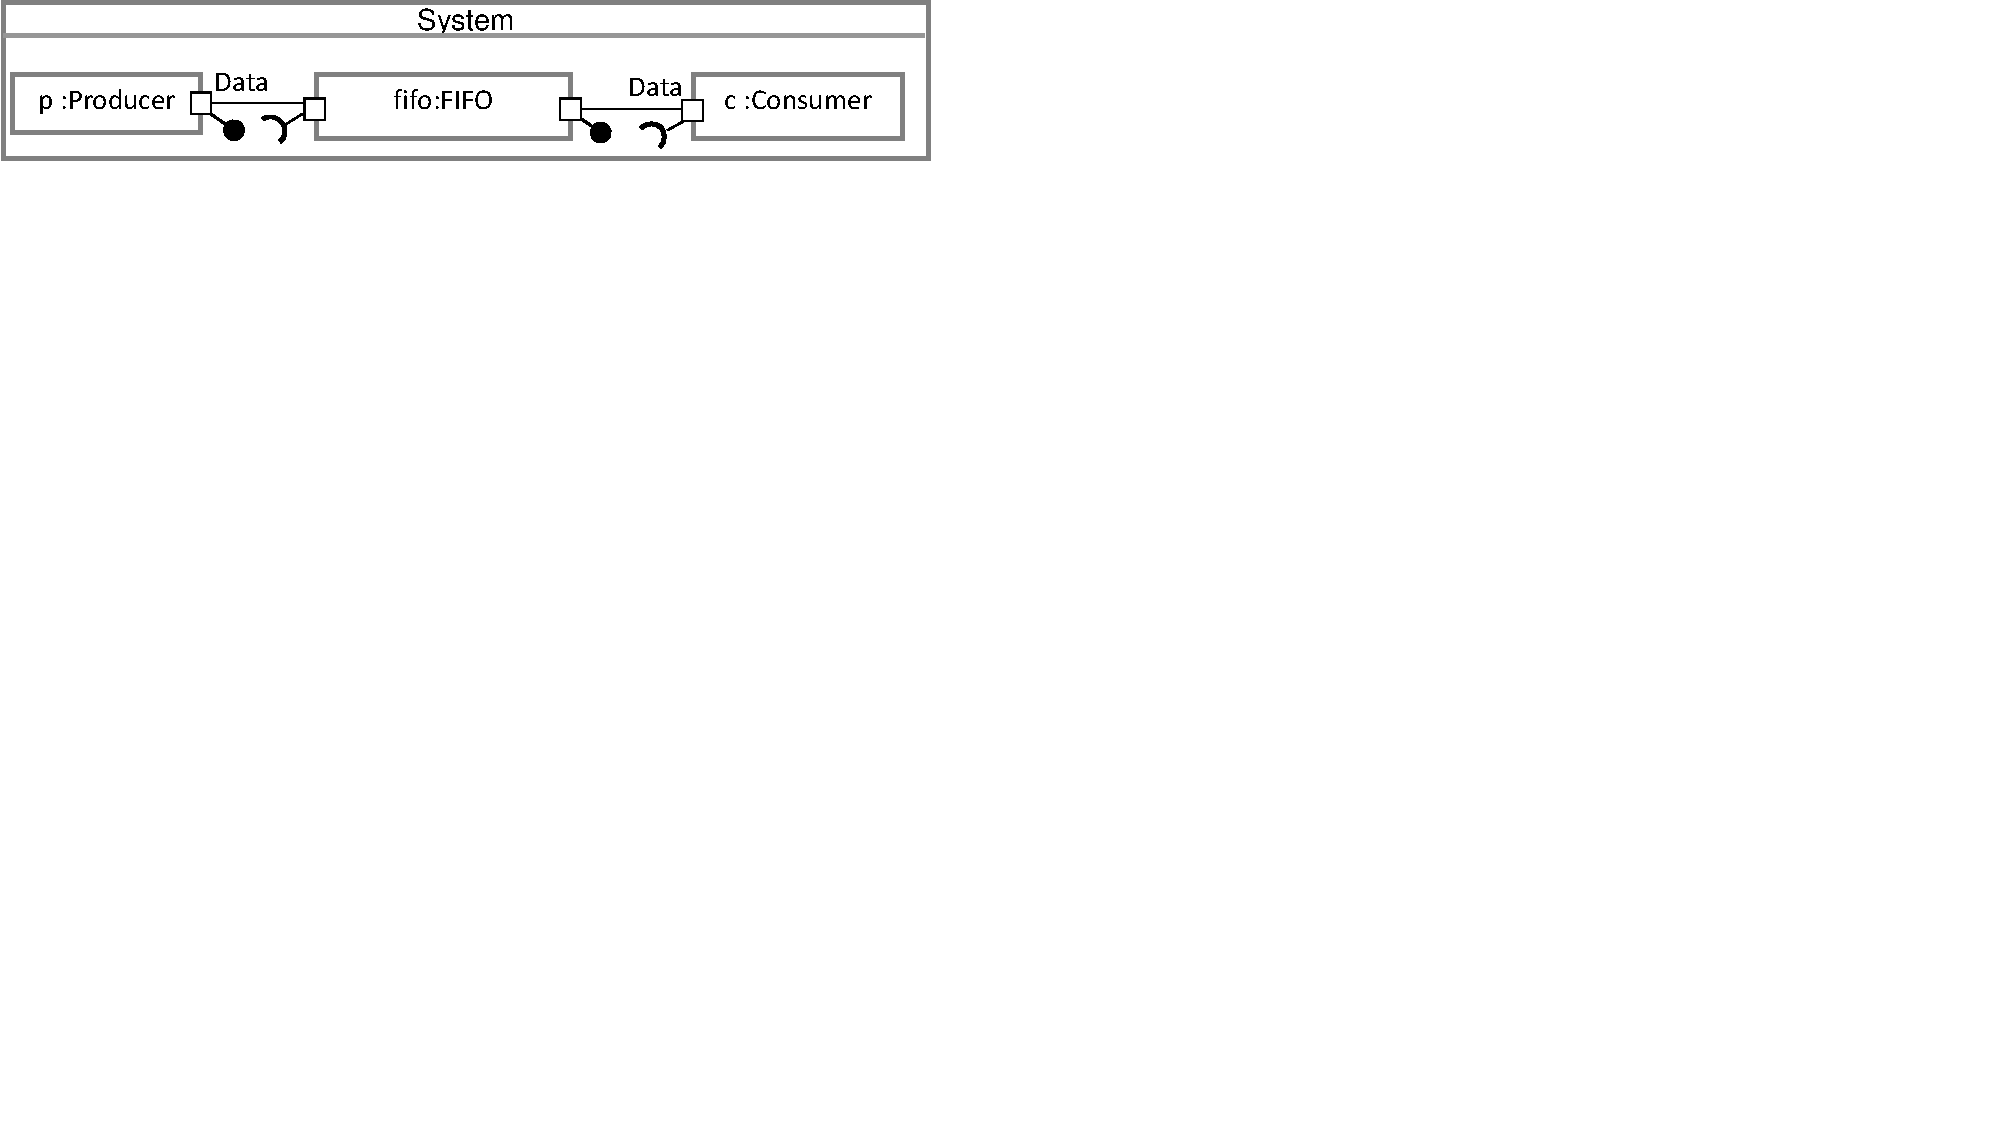
\includegraphics[clip, trim=0cm 16.3cm 17.6cm 0cm, width=\columnwidth]{figures/dataportexample.pdf}
	\caption{Component-based architecture example with data port} 
	\label{fig:dataportexample}
\end{comment}


\begin{minipage}{\columnwidth}
	\lstinputlisting[language=C++, caption={System using data ports}, label=lst:dataport,frame=f]{
		code/dataport.cpp
		}
\end{minipage} 

In implementation, the producer provides data items to the fifo via the port \ttt{pProvideData} by calling \ttt{pProvideData->sendSignal(item)} (line 6) as an object-oriented way.
In case that the behavior of the component is described by a state machine, the \ttt{sendSignal} method will fire a signal event in order for the state machine to handle it.







We have presented how XSeparation works for the architecture structure.
In the next section, XSeparation for the architecture behavior described by UML State Machines will be detailed.